\documentclass[12pt,twoside]{article}

\newcommand{\reporttitle}{Project 2: Advanced Lane Detection}
\newcommand{\reportauthor}{Thomas Teh}
\newcommand{\reporttype}{Project Report}
\newcommand{\cid}{0124 3008}

% include files that load packages and define macros
%%%%%%%%%%%%%%%%%%%%%%%%%%%%%%%%%%%%%%%%%
% University Assignment Title Page 
% LaTeX Template
% Version 1.0 (27/12/12)
%
% This template has been downloaded from:
% http://www.LaTeXTemplates.com
%
% Original author:
% WikiBooks (http://en.wikibooks.org/wiki/LaTeX/Title_Creation)
%
% License:
% CC BY-NC-SA 3.0 (http://creativecommons.org/licenses/by-nc-sa/3.0/)
% 
% Instructions for using this template:
% This title page is capable of being compiled as is. This is not useful for 
% including it in another document. To do this, you have two options: 
%
% 1) Copy/paste everything between \begin{document} and \end{document} 
% starting at \begin{titlepage} and paste this into another LaTeX file where you 
% want your title page.
% OR
% 2) Remove everything outside the \begin{titlepage} and \end{titlepage} and 
% move this file to the same directory as the LaTeX file you wish to add it to. 
% Then add \input{./title_page_1.tex} to your LaTeX file where you want your
% title page.
%
%----------------------------------------------------------------------------------------
%	PACKAGES AND OTHER DOCUMENT CONFIGURATIONS
%----------------------------------------------------------------------------------------
\usepackage{ifxetex}
\usepackage{textpos}
%\usepackage{natbib}
%\usepackage{breqn}
\usepackage{kpfonts}
\usepackage[a4paper,hmargin=2.8cm,vmargin=2.0cm,includeheadfoot]{geometry}
\usepackage{ifxetex}
\usepackage{stackengine}
\usepackage{tabularx,longtable,multirow,subfigure,caption}%hangcaption
\usepackage{fncylab} %formatting of labels
\usepackage{fancyhdr}
\usepackage{color}
\usepackage[tight,ugly]{units}
\usepackage{url}
\usepackage{float}
\usepackage[english]{babel}
\usepackage{amsmath}
\usepackage{graphicx}
\usepackage[colorinlistoftodos]{todonotes}
\usepackage{dsfont}
\usepackage{epstopdf} % automatically replace .eps with .pdf in graphics
\usepackage{natbib}
\usepackage{backref}
\usepackage{array}
\usepackage{latexsym}
\usepackage{etoolbox}
\usepackage{algorithmic}
\usepackage[]{algorithm2e}

\usepackage{enumerate} % for numbering with [a)] format 



\ifxetex
\usepackage{fontspec}
\setmainfont[Scale=.8]{OpenDyslexic-Regular}
\else
\usepackage[pdftex,pagebackref,hypertexnames=false,colorlinks]{hyperref} % provide links in pdf
\hypersetup{pdftitle={},
  pdfsubject={}, 
  pdfauthor={\reportauthor},
  pdfkeywords={}, 
  pdfstartview=FitH,
  pdfpagemode={UseOutlines},% None, FullScreen, UseOutlines
  bookmarksnumbered=true, bookmarksopen=true, colorlinks,
    citecolor=black,%
    filecolor=black,%
    linkcolor=black,%
    urlcolor=black}
\usepackage[all]{hypcap}
\fi

\usepackage{tcolorbox}
\usepackage{hyperref}
% various theorems
\usepackage{ntheorem}
\theoremstyle{break}
\newtheorem{lemma}{Lemma}
\newtheorem{theorem}{Theorem}
\newtheorem{remark}{Remark}
\newtheorem{definition}{Definition}
\newtheorem{proof}{Proof}

% example-environment
\newenvironment{example}[1][]
{ 
\vspace{4mm}
\noindent\makebox[\linewidth]{\rule{\hsize}{1.5pt}}
\textbf{Example #1}\\
}
{ 
\noindent\newline\makebox[\linewidth]{\rule{\hsize}{1.0pt}}
}



%\renewcommand{\rmdefault}{pplx} % Palatino
% \renewcommand{\rmdefault}{put} % Utopia

\ifxetex
\else
\renewcommand*{\rmdefault}{bch} % Charter
\renewcommand*{\ttdefault}{cmtt} % Computer Modern Typewriter
%\renewcommand*{\rmdefault}{phv} % Helvetica
%\renewcommand*{\rmdefault}{iwona} % Avant Garde
\fi

\setlength{\parindent}{0em}  % indentation of paragraph

\setlength{\headheight}{14.5pt}
\pagestyle{fancy}
\fancyfoot[ER,OL]{\thepage}%Page no. in the left on
                                %odd pages and on right on even pages
\fancyfoot[OC,EC]{\sffamily }
\renewcommand{\headrulewidth}{0.1pt}
\renewcommand{\footrulewidth}{0.1pt}
\captionsetup{margin=10pt,font=small,labelfont=bf}


%--- chapter heading

\def\@makechapterhead#1{%
  \vspace*{10\p@}%
  {\parindent \z@ \raggedright %\sffamily
        %{\Large \MakeUppercase{\@chapapp} \space \thechapter}
        %\\
        %\hrulefill
        %\par\nobreak
        %\vskip 10\p@
    \interlinepenalty\@M
    \Huge \bfseries 
    \thechapter \space\space #1\par\nobreak
    \vskip 30\p@
  }}

%---chapter heading for \chapter*  
\def\@makeschapterhead#1{%
  \vspace*{10\p@}%
  {\parindent \z@ \raggedright
    \sffamily
    \interlinepenalty\@M
    \Huge \bfseries  
    #1\par\nobreak
    \vskip 30\p@
  }}
  



% %%%%%%%%%%%%% boxit
\def\Beginboxit
   {\par
    \vbox\bgroup
	   \hrule
	   \hbox\bgroup
		  \vrule \kern1.2pt %
		  \vbox\bgroup\kern1.2pt
   }

\def\Endboxit{%
			      \kern1.2pt
		       \egroup
		  \kern1.2pt\vrule
		\egroup
	   \hrule
	 \egroup
   }	

\newenvironment{boxit}{\Beginboxit}{\Endboxit}
\newenvironment{boxit*}{\Beginboxit\hbox to\hsize{}}{\Endboxit}



\allowdisplaybreaks

\makeatletter
\newcounter{elimination@steps}
\newcolumntype{R}[1]{>{\raggedleft\arraybackslash$}p{#1}<{$}}
\def\elimination@num@rights{}
\def\elimination@num@variables{}
\def\elimination@col@width{}
\newenvironment{elimination}[4][0]
{
    \setcounter{elimination@steps}{0}
    \def\elimination@num@rights{#1}
    \def\elimination@num@variables{#2}
    \def\elimination@col@width{#3}
    \renewcommand{\arraystretch}{#4}
    \start@align\@ne\st@rredtrue\m@ne
}
{
    \endalign
    \ignorespacesafterend
}
\newcommand{\eliminationstep}[2]
{
    \ifnum\value{elimination@steps}>0\leadsto\quad\fi
    \left[
        \ifnum\elimination@num@rights>0
            \begin{array}
            {@{}*{\elimination@num@variables}{R{\elimination@col@width}}
            |@{}*{\elimination@num@rights}{R{\elimination@col@width}}}
        \else
            \begin{array}
            {@{}*{\elimination@num@variables}{R{\elimination@col@width}}}
        \fi
            #1
        \end{array}
    \right]
    & 
    \begin{array}{l}
        #2
    \end{array}
    &%                                    moved second & here
    \addtocounter{elimination@steps}{1}
}
\makeatother

%% Fast macro for column vectors
\makeatletter  
\def\colvec#1{\expandafter\colvec@i#1,,,,,,,,,\@nil}
\def\colvec@i#1,#2,#3,#4,#5,#6,#7,#8,#9\@nil{% 
  \ifx$#2$ \begin{bmatrix}#1\end{bmatrix} \else
    \ifx$#3$ \begin{bmatrix}#1\\#2\end{bmatrix} \else
      \ifx$#4$ \begin{bmatrix}#1\\#2\\#3\end{bmatrix}\else
        \ifx$#5$ \begin{bmatrix}#1\\#2\\#3\\#4\end{bmatrix}\else
          \ifx$#6$ \begin{bmatrix}#1\\#2\\#3\\#4\\#5\end{bmatrix}\else
            \ifx$#7$ \begin{bmatrix}#1\\#2\\#3\\#4\\#5\\#6\end{bmatrix}\else
              \ifx$#8$ \begin{bmatrix}#1\\#2\\#3\\#4\\#5\\#6\\#7\end{bmatrix}\else
                 \PackageError{Column Vector}{The vector you tried to write is too big, use bmatrix instead}{Try using the bmatrix environment}
              \fi
            \fi
          \fi
        \fi
      \fi
    \fi
  \fi 
}  
\makeatother

\robustify{\colvec}

%%% Local Variables: 
%%% mode: latex
%%% TeX-master: "notes"
%%% End: 
 % various packages needed for maths etc.
% quick way of adding a figure
\newcommand{\fig}[3]{
 \begin{center}
 \scalebox{#3}{\includegraphics[#2]{#1}}
 \end{center}
}

%\newcommand*{\point}[1]{\vec{\mkern0mu#1}}
\newcommand{\ci}[0]{\perp\!\!\!\!\!\perp} % conditional independence
\newcommand{\point}[1]{{#1}} % points 
\renewcommand{\vec}[1]{{\boldsymbol{{#1}}}} % vector
\newcommand{\mat}[1]{{\boldsymbol{{#1}}}} % matrix
\newcommand{\R}[0]{\mathds{R}} % real numbers
\newcommand{\Z}[0]{\mathds{Z}} % integers
\newcommand{\N}[0]{\mathds{N}} % natural numbers
\newcommand{\nat}[0]{\mathds{N}} % natural numbers
\newcommand{\Q}[0]{\mathds{Q}} % rational numbers
\ifxetex
\newcommand{\C}[0]{\mathds{C}} % complex numbers
\else
\newcommand{\C}[0]{\mathds{C}} % complex numbers
\fi
\newcommand{\tr}[0]{\text{tr}} % trace
\renewcommand{\d}[0]{\mathrm{d}} % total derivative
\newcommand{\inv}{^{-1}} % inverse
\newcommand{\id}{\mathrm{id}} % identity mapping
\renewcommand{\dim}{\mathrm{dim}} % dimension
\newcommand{\rank}[0]{\mathrm{rk}} % rank
\newcommand{\determ}[1]{\mathrm{det}(#1)} % determinant
\newcommand{\scp}[2]{\langle #1 , #2 \rangle}
\newcommand{\kernel}[0]{\mathrm{ker}} % kernel/nullspace
\newcommand{\img}[0]{\mathrm{Im}} % image
\newcommand{\idx}[1]{{(#1)}}
\DeclareMathOperator*{\diag}{diag}
\newcommand{\E}{\mathds{E}} % expectation
\newcommand{\var}{\mathds{V}} % variance
\newcommand{\gauss}[2]{\mathcal{N}\big(#1,\,#2\big)} % gaussian distribution N(.,.)
\newcommand{\gaussx}[3]{\mathcal{N}\big(#1\,|\,#2,\,#3\big)} % gaussian distribution N(.|.,.)
\newcommand{\gaussBig}[2]{\mathcal{N}\left(#1,\,#2\right)} % see above, but with brackets that adjust to the height of the arguments
\newcommand{\gaussxBig}[3]{\mathcal{N}\left(#1\,|\,#2,\,#3\right)} % see above, but with brackets that adjust to the height of the arguments
\DeclareMathOperator{\cov}{Cov} % covariance (matrix) 
\ifxetex
\renewcommand{\T}[0]{^\top} % transpose
\else
\newcommand{\T}[0]{^\top}
\fi
% matrix determinant
\newcommand{\matdet}[1]{
\left|
\begin{matrix}
#1
\end{matrix}
\right|
}



%%% various color definitions
\definecolor{darkgreen}{rgb}{0,0.6,0}

\newcommand{\blue}[1]{{\color{blue}#1}}
\newcommand{\red}[1]{{\color{red}#1}}
\newcommand{\green}[1]{{\color{darkgreen}#1}}
\newcommand{\orange}[1]{{\color{orange}#1}}
\newcommand{\magenta}[1]{{\color{magenta}#1}}
\newcommand{\cyan}[1]{{\color{cyan}#1}}


% redefine emph
\renewcommand{\emph}[1]{\blue{\bf{#1}}}

% place a colored box around a character
\gdef\colchar#1#2{%
  \tikz[baseline]{%
  \node[anchor=base,inner sep=2pt,outer sep=0pt,fill = #2!20] {#1};
    }%
}%
 % short-hand notation and macros
\DontPrintSemicolon

%%%%%%%%%%%%%%%%%%%%%%%%%%%%

\begin{document}
% front page
% Last modification: 2016-09-29 (Marc Deisenroth)
\begin{titlepage}

\newcommand{\HRule}{\rule{\linewidth}{0.5mm}} % Defines a new command for the horizontal lines, change thickness here


%----------------------------------------------------------------------------------------
%	LOGO SECTION
%----------------------------------------------------------------------------------------

%
\includegraphics[width = 4cm]{./figures/imperial}\\[0.5cm] 

\begin{center} % Center remainder of the page

%----------------------------------------------------------------------------------------
%	HEADING SECTIONS
%----------------------------------------------------------------------------------------
\textsc{\LARGE \reporttype}\\[1.5cm] 
\textsc{\Large Udacity}\\[0.5cm] 
\textsc{\large Self-Driving Car Nanodegree}\\[0.5cm] 
%----------------------------------------------------------------------------------------
%	TITLE SECTION
%----------------------------------------------------------------------------------------

\HRule \\[0.4cm]
{ \huge \bfseries \reporttitle}\\ % Title of your document
\HRule \\[1.5cm]
\end{center}
%----------------------------------------------------------------------------------------
%	AUTHOR SECTION
%----------------------------------------------------------------------------------------

%\begin{minipage}{0.4\hsize}
\begin{flushleft} \large
\textsc{Author:}\\
\reportauthor~%(CID: \cid) % Your name
\end{flushleft}
\vspace{2cm}
\makeatletter
Date: \@date 

\vfill % Fill the rest of the page with whitespace



\makeatother


\end{titlepage}




%%%%%%%%%%%%%%%%%%%%%%%%%%%% Main document
\section{Introduction}
This project is part of the Self-Driving Car Nanodegree by Udacity and its objective is to build an advanced lane detection algorithm. The pipeline for the algorithm is as follow:
\begin{enumerate}
	\item \textbf{Calibration and distortion correction: } Compute the camera calibration matrix and distortion coefficients using chessboard images, which we then use to correct the distortion of the raw images from the camera.
	\item \textbf{Perspective transformation:}  Select the region of interest in the raw images and apply a perspective transform ("birds-eye view")
	\item \textbf{Preprocessing and construct binary images:} Preprocessing the images and construct binary images using the gradients and color transforms.
	\item \textbf{Lane detection:} Apply histogram and sliding window on the first frame of video. Subsequent frames are fitted and smoothed based on the first frame.
	\item \textbf{Curvature estimation:} Determine the curvature of the lane and the vehicle center with respect to the lane center
	\item \textbf{Overlay the detected lane:} Visual display of the lane boundaries and numerical curvature and vehicle position.
\end{enumerate}

\section{Pipeline}
\subsection{Calibration and Distortion Correction}
We calibrate the camera using chessboard images provided. Using OpenCV function findChessBoardCorners(), we automatically find corners in an image of a chessboard pattern. 

\begin{figure}[H]
	\begin{center}
		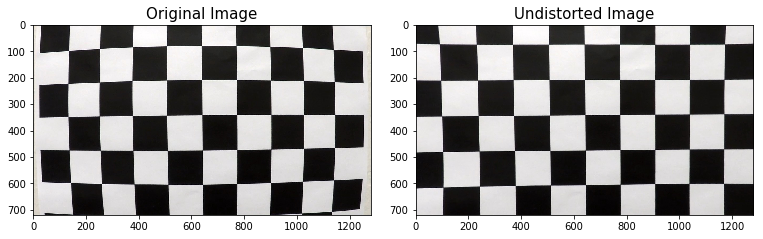
\includegraphics[width = 1.0\hsize]{./figures/Calibration.png} 
		\caption{Camera distortion correction using chessboard images.} % caption of the figure
		\label{fig:chessboard} % a label. When we refer to this label from the text, the figure %number is included automatically
	\end{center}
\end{figure}

Then we calibrate the camera given the object points, image points and image shape using the function calibrateCamera(). Finally we use the undistort() function. The sample source image and the undistorted image of the chessboard and raw image are in Figure \ref{fig:chessboard} and \ref{fig:cameraundistort} respectively. Detailed implementation is in Calibration.py.

\begin{figure}[H]
	\begin{center}
		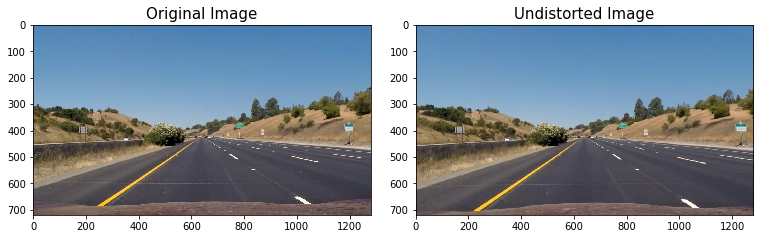
\includegraphics[width = 1.0\hsize]{./figures/Undistorted.png} 
		\caption{Raw images before and after distortion correction.} % caption of the figure
		\label{fig:cameraundistort} % a label. When we refer to this label from the text, the figure %number is included automatically
	\end{center}
\end{figure}


\subsection{Perspective Transform}

\begin{figure}[H]
	\begin{center}
		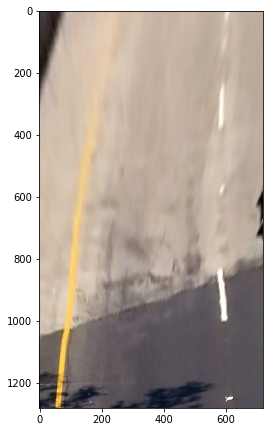
\includegraphics[width = 0.4\hsize]{./figures/Warped.png} 
		\caption{Image after applying perspective transform to a region of interest.} % caption of the figure
		\label{fig:posttransform} % a label. When we refer to this label from the text, the figure %number is included automatically
	\end{center}
\end{figure}

We applied OpenCV functions getPerspectiveTransform() and warpPerspective() to map the points in a given image to different image points with the bird's eye view perspective. The source points are manually determined and this would lead to a major weakness in our lane detection algorithm, which we will discuss later. 

The image after the transform is shown in Figure \ref{fig:posttransform}. The detailed implementation is found in Warp.py





\subsection{Preprocessing and Constructing Binary Images}

\begin{figure}[H]
	\begin{center}
		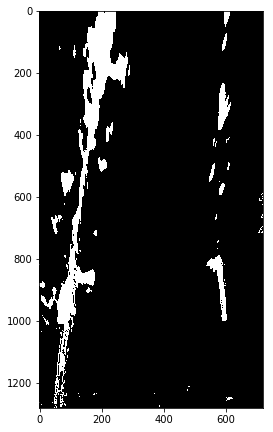
\includegraphics[width = 0.4\hsize]{./figures/Threshold.png} 
		\caption{Binary image after applying the relevant thresholds to selected metrics.} % caption of the figure
		\label{fig:binaryimage} % a label. When we refer to this label from the text, the figure %number is included automatically
	\end{center}
\end{figure} 
We construct the binary images using a combination of two different methods - gradients and color transforms. Before we compute the gradient, the raw images is preprocessed using the following:
\begin{itemize}
	\item Contrast Limited Adaptive Histogram Equalization (CLAHE) is applied on each of the RGB channels of the raw image. 
	\item Gaussian Smoothing is used to smoothed out the images.
	\item Lastly, we convert the the image from RGB to HLS and extract the S channel.
\end{itemize}
The gradients of the image's S channel, across the x and y axes, are then computed using OpenCV function Sobel(). We only normalize the gradients and take only the absolute values. While in the implementation, we computed the gradient magnitude and direction, however, it is found that constructing the binary images using those metrics are not great. \\

For the color transforms, we convert the raw BGR image into LUV and LAB channels respectively. We then extract the L and B channels respectively. Now, we are ready to construct the binary images.\\

We apply the following thresholds:
\begin{center}
	\begin{tabular}{|c|c|c|}
	\hline
	Metrics							&			Lower Bound			& 			Upper Bound\\\hline
	Gradient along x-axis	&			40						&			100\\
	Gradient along y-axis	&			40						&			100\\
	L channel						&			200						&			255\\
	B channel						&			150						&			200\\\hline
	\end{tabular}
\end{center}

We retain pixels that meet falls within the thresholds for any of the above metrics in order to construct the binary image. A sample binary image in shown in Figure  \ref{fig:binaryimage}.


Detailed implementation of the preprocessing and construction of the binary images can be found in Thresholding.py.

\subsection{Lane Detection}
\begin{figure}[H]
	\begin{center}
		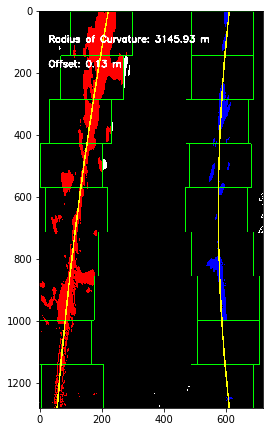
\includegraphics[width = 0.4\hsize]{./figures/LaneDetection.png} 
		\caption{Detected Lanes.} % caption of the figure
		\label{fig:detection} % a label. When we refer to this label from the text, the figure %number is included automatically
	\end{center}
\end{figure} 

The lane detection algorithm is divided into primary and secondary detection. Primary detection is used for single image or the first frame of the video. Secondary detection relies on the fact that we have already detected the lanes in the previous frames and reuse the polynomial functions again.\\

\textbf{Primary Detection: } We construct a histogram by adding the pixels at each column of the x-axis. If we have a line, it is more likely for us to get 1s in that region, hence we should have a peak. Since there are left and right lanes, we would expect the histogram to be bimodal (this assumption will be challenged later). Starting from the bottom of the peak in the histogram, we use a sliding window placed around the line centers to find and follow the lines up to the top of the frame. Once we have identify all the relevant pixels, we can then fit a quadratic line across the pixels.\\

\textbf{Secondary Detection: } Primary detection is computationally expensive. When the car is on the road, we need the lane detection to be as efficient and quick as possible. Hence, once we know where the lanes are in the prior frames, we can make use of that information. \\

We can start searching a customized regions formed by the two polynomial functions fitted in the previous frame. 
If we found there are more than 50 pixels, we would then refit the line; else we will use the previously fitted line.

A sample of the lane detected is shown in Figure \ref{fig:detection}.



\subsection{Curvature Estimation}

The formula for radius of curvature at any point $x$ for the curve $y = f(x)$ is given by:
\begin{align*}
R & = \frac{\left[1 + \left(\frac{dy}{dx}\right)^2\right]^\frac{3}{2}}{\left\vert \frac{d^2y}{dx^2}\right\vert}.
\end{align*}

Since in our case, we are fitting in quadratic curve, hence the derivatives of the function can be found easily. Thus we can compute the radius of curvature easily. Once we obtain the curvature of the left and right boundary of the lane, we can then compute the lane center. \\

Assuming that the camera is mounted at the center of the car, hence the center of the car is just half the image size. We can then compute the difference between the car center and the lane center to know how much the car is drifting from the center.


\subsection{Visualization}
The output of the lane detection algorithms for the highway video and the challenge video can be found in
\begin{itemize}
	\item \url{https://youtu.be/JSLnoQthI5M}
	\item \url{https://youtu.be/iPrrPCVpwKU}
\end{itemize}

\newpage

\section{Major Pitfalls and Potential Improvements}
From the videos, we can see that the algorithm works well for roads with relatively few curves. However, once the car is on a winding road with a lot of turns, the algorithm fails. There are a few issues with the existing algorithm.

\begin{enumerate}
	\item Secondary detection fails if the algorithm fails to detect the lanes at one of the frames. This can be solve by making the algorithm to do the primary detection whenever the curvature of the curves is below a certain level (in our case, 1000). The rationale is that when the radius of curvature is small, it implies a sharp turn or bend. It is best at the moment to run the primary detection when there are plenty of bends.
	
	\item Perhaps the biggest issue is that the region of interest in the camera is dynamic. When the car is on a relatively straight road, the region of interest (i.e. where the lanes are), are relatively stable. However, as seen in the challenge video, on a window, the region of interest is less well-behaved. In extreme cases, the lanes actually start at the side of the image instead of from the bottom. If we do not overcome this particular issue, it will be difficult to ensure that the car stays in lane all the timee.
\end{enumerate}

\subsection{Can we shoot two birds with one stone?}
One potential solution to a dynamic region of interest is image segmentation. While the car is on the road, the ability to know the surroundings objects can be vital. Hence, we also need an algorithm to implement image segmentation and recognition.\\

We can potentially implement image segmentation algorithm with a convolutional neural network. We can then implement the lane finding algorithm once we can detect the road dynamically in an image. 









%\bibliography{reference}
%\bibliographystyle{apalike}


\end{document}
%%% Local Variables: 
%%% mode: latex
%%% TeX-master: t
%%% End: 
